\documentclass[../../main.tex]{subfiles}
 
\begin{document}

\begin{table}
\small
\centering
\begin{tabular}{| c | c | c | c |}
\hline \hline
Question & COSC330 $N$ & COSC330 Mean & COSC330 Std. dev. \\ \hline
10 & 8 & 3.13 & 1.46 \\ \hline
11 & 8 & 3.71 & 1.38 \\ \hline
12 & 8 & 3.75 & 1.04 \\ \hline
13 & 8 & 3.25 & 1.39 \\ \hline
14 & 8 & 3.63 & 1.19 \\ \hline
15 & 8 & 3.86 & 0.69 \\ \hline
16 & 8 & 3.29 & 1.25 \\ \hline
\hline
\end{tabular}
\caption{\label{tab:courses:adv_eval_1} Summary of questions 10-16 on the student evaluation form, for COSC330/PHYS306, taught in Spring 2018.  These questions pertain to the \textit{course}. $N$ refers to the number of students.}
\end{table}

\begin{table}
\centering
\begin{tabular}{| c | c | c | c |}
\hline \hline
Question & COSC330 $N$ & COSC330 Mean & COSC330 Std. dev. \\ \hline
17 & 8 & 3.38 & 1.60 \\ \hline
18 & 8 & 3.50 & 1.20 \\ \hline
19 & 8 & 3.13 & 1.46 \\ \hline
20 & 8 & 4.25 & 0.71 \\ \hline
21 & 8 & 3.50 & 1.41 \\ \hline
22 & 8 & 4.00 & 0.89 \\ \hline
23 & 8 & 4.25 & 1.16 \\ \hline
24 & 8 & 4.29 & 1.25 \\ \hline
25 & 8 & 2.88 & 1.36 \\ \hline
\hline
\end{tabular}
\caption{\label{tab:courses:adv_eval_2} Summary of questions 17-25 on the student evaluation form, for COSC330/PHYS306, taught in Spring 2018.  These questions pertain to the \textit{professor}. $N$ refers to the number of students.}
\end{table}

Tables \ref{tab:courses:adv_eval_1} and \ref{tab:courses:adv_eval_2} show the results of my advanced computer science and physics course.  For the lower scores, the fractional error is about 50\%, whereas the higher scores have fractional error of about 20\%, similar to the introductory courses (see Appendix). The numbers inform the analysis of my teaching of COSC330, and the students' remarks in the evaluations provide more detail. \\ \hspace{0.1cm}

Some students remarked that the course did not seem adequately structured or prepared.  This was in large part caused by the disruption of not having the equipment I needed.  Although I did order the textbooks and digital components long before the first day of class, the company shipping the parts refused to accept our department cheque, wanting a credit card.  I had chosen a standard electronics textbook and lab companion book written by professors at MIT \cite{theArtOfElectronics} which assumed we would have the parts. Upon hearing that the parts would be delayed, I was forced to revert to an alternative textbook a colleague provided me \cite{digitalFund}. This text was excellent for demonstrations of binary math and boolean algebra, but was lighter on hardware. The students were unhappy that the textbooks they bought would not be used until later in the course. \\ \hspace{0.1cm}

We now have the reusable digital components stored in the physics labs, so we will be able to integrate the lab and lecture activities and use free instructor desk copies of the MIT text I obtained.  Also, this will allow me to do what I originally planned, which was to organize the course by \textit{sub-topic} rather than simply doing all the mathematics first.  This should raise the students' assessment of categories like course preparation and effective use of class time.  Further, pre-assembly of some of the digital circuits will facilitate learning by freeing up time to probe how the circuit projects work (taking it apart and reassembling, for example). \\ \hspace{0.1cm}

Having experienced once how long it takes students to assemble circuits, I can better plan future class times.  Students remarked that the super heterodyne AM radio took too long to assemble, for example.  In the future, those projects could be partially assembled by me in advance.  Some students also wrote that they didn't understand how the transistor radio was related to digital circuits.  I included the transistor radio so the students could get a hands-on experience working with transistors, which form the basis for other all other digital components.  In the next iteration of the course, partial pre-assembly should leave more time to probe how the circuit works using transistors, rather than spending more time just building the project.  \\ \hspace{0.1cm}

Some students remarked that they felt under-prepared for the course material.  I did notice that I had two Whittier Scholar Program majors (F. Capraro, and A. Dodds), and while one felt the course was easy and appeared comfortable with the material, the other did not.  Nevertheless, I was pleased to have those students and would like to encourage WSP enrollment in the future.  To entice the curiosity of the WSP majors, I included some cross-disciplinary examples during the Boolean algebra phase of the course.  Nevertheless, the pace will have to be relaxed if I am to continue to accomodate WSP majors in this type of course.  Some 3-2 engineering and mathematics majors felt that they did not remember the physics related to sub-topics like resistors and capacitors well enough to relate those concepts to transistors.  I had a tough decision regarding the course prerequisites, which are normally introductory-level physics and computer science courses.  My department and I felt that in the course's inaugural year that I should waive the prerequisites on a case-by-case basis in order to gain more students.  I promoted COSC330 in PHYS150 and PHYS180, and students who felt they could handle it approached me. It turned out to be the mathematics seniors who did not remember the physics and struggled with circuit-based topics, which is taught in PHYS180 (a course they might not have taken).  In the future, I plan to review circuit analysis in more detail, before adding digital elements. \\ \hspace{0.1cm}

%\begin{figure}
%\centering
%\includegraphics[width=0.33\textwidth,angle=270]{aggregate_data_spring_2018_adv.eps}
%\caption{\label{fig:ag_data2} Aggregate standard deviations versus mean scores for questions 10-25 for advanced courses taught in Spring 2018.}
%\end{figure}

\end{document}